\documentclass[a4paper,titlepage]{scrartcl}
\pagestyle{plain}
\usepackage[utf8]{inputenc}
\usepackage[T1]{fontenc}
\usepackage[german]{babel}
\usepackage{float}
\usepackage{graphicx}
\usepackage{amsmath,amssymb,amstext}
\usepackage{enumerate}
\usepackage{units}

\numberwithin{equation}{section}

\title{Versuch P2-11: Polarisation und Doppelbrechung\\Vorbereitung}
\author{Gruppe Di-22\\Genti Saliu, Jonas Müller}
\date{15. Juni 2014}

\begin{document}
	\begin{titlepage}
		\maketitle
		\thispagestyle{empty}
	\end{titlepage}
	
\newpage
\pagenumbering{roman}
\tableofcontents

\newpage
\pagenumbering{arabic}

\section{Theoretische Grundlagen}

\subsection{Transversalwelle}
Eine Transversalwelle ist eine physikalische Welle, bei der eine Schwingung senkrecht zu ihrer Ausbreitungsrichtung erfolgt \cite{wiki:transversal}.

\subsection{Longitudinalwelle}
Eine Longitudinalwelle ist eine physikalische Welle, die in Ausbreitungsrichtung schwingt \cite{wiki:longitudinal}.

\subsection{Polarisation}
In der klassischen Elektrodynamik wird Licht als \emph{transversale elektromagnetische Welle} aufgefasst, deren Amplitude durch den Vektor des elektrischen Feldes $\vec{E}$ oder des Magnetfeldes $\vec{B}$ gegeben ist. Die Ausbreitungsrichtung verläuft über den Vektor $\vec{k}$. $\vec{k}$, $\vec{E}$ und $\vec{B}$ sind zueinander orthogonal.\\ \\
Die Richtung des $\vec{E}$-Feld-Vektors wird Polarisationsrichtung genannt. Die Polarisation beschreibt definitionsgemäß die Richtung der Schwingung einer Transversalwelle. Ändert sich diese Richtung schnell und ungeordnet, spricht man von einer unpolarisierten Welle. Bei Longitudinalwellen gibt es keine Polarisation.
\begin{figure}[H]
	\centering
	\begin{tabular}{@{}r@{}}
		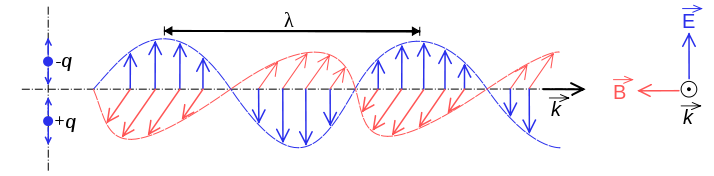
\includegraphics[width=0.8\textwidth]{bilder/licht.png}\\
		\footnotesize\sffamily\textbf{Quelle:} Wikipedia \cite{wiki:licht}
	\end{tabular}
	\caption{Licht als elektromagnetische Welle}
	\label{fig:licht}
\end{figure}
Man unterscheidet drei Arten von Polarisation:
\begin{itemize}
\item \textbf{lineare Polarisation}: die Richtung der Schwingung ist konstant, lediglich die Auslenkung aus der Ruhelage ändert periodisch ihren Betrag und Vorzeichen.
\item \textbf{zirkulare Polarisation}: der Betrag der Schwingung ist konstant, ihre Richtung ändert sich innerhalb der senkrecht zum Wellenvektor stehenden Ebene mit konstanter Winkelgeschwindigkeit.
\item \textbf{elliptische Polarisation}: dies ist eine Mischform aus den beiden vorhin betrachteten Polarisationsarten.
\end{itemize}
Licht kann mithilfe von Polarisatoren mit verschiedenen Mechanismen polarisiert werden, durch Dichroismus, Reflexion, Doppelbrechung, Streuung und Beugung. Wie Polarisation durch Doppelbrechung funktioniert, werden wir im nachfolgenden Abschnitt behandeln. Polarisatoren, die eine linear polarisierte elektromagnetische Welle erzeugen, werden Linearpolarisatoren genannt, die die zirkular polarisiertes Licht erzeugen, Zirkularpolarisator \cite{wiki:polarisator}.\\ \\
Polarisatoren sind also Bauteile, die Licht mit einer bestimmten Polarisation aus nicht, teilweise oder anders polarisierten elektromagnetischen Wellen, herasfiltern.\\ \\
Ein Polarisator, der dazu benutzt wird vorhandene Polarisation festzustellen oder zu messen, heißt Analysator.

\subsection{Polarisation durch Dichroismus}
Bestimmte Materialen (hauptsächlich Kristalle) sind in der Lage Licht in Abhängigkeit von der Polarisation unterschiedlich stark zu absorbieren. Das macht sich auf deren Reflexionsverhalten bemerkbar. Diese Materiale haben eine oder mehrere ausgezeichnete optische Achsen. Bei einachsigen Materialen wird einfallendes Licht je nach Polarisation in einem ordentlichen und einem außerordentlichen Strahl aufgespalten. Je nachdem, ob der ordentliche oder außerordentliche Strahl stärker bzw. schwächer absorbiert wird, spricht man von einem dichroitischen Kristall. Dieser Effekt ist stark wellenlängenspezifisch, bei anderen Wellenlängen des Lichts tritt der Effekt der Absorption nicht mehr, sondern Doppelbrechung, worauf nachfolgend näher eingegangen wird \cite{wiki:dichroismus}.

\subsection{Polarisation durch Streuung}
Fällt unpolarisiertes Licht auf ein streuendes Medium, so ist das Streulicht, das das Medium senkrecht zur Einfallsrichtung verlässt, linear polarisiert. Die elektromagnetische Welle des Lichtes kommt zu einer Wechselwirkung mit den Molekülen/Atomen, die zu Dipolschwingungen angeregt werden. Das von den Molekülen in Vorwärtsrichtung gestreute Licht bleibt unpolarisiert, senkrecht zur Strahlrichtung tritt die maximale Polarisation des Lichtes auf, denn die Abstrahlung erfolgt senkrecht zur Schwingungsrichtung der Moleküldipole.

\subsection{Polarisation durch Reflexion}
Wenn unpolarisiertes Licht unter dem Brewster-Winkel\footnote{Der Winkel, bei dem von einem einfallenden, unpolarisierten Licht nur die senkrecht zur Einfallsebene polarisierten Anteile reflektiert werden} auf eine Glasplatte fällt, ist der reflektierte Teil senkrecht zur Einfallsebene des Lichtes linear polarisiert, der transmittierte Anteil ist jedoch nur teileweise polarisiert. Indem man dieses Licht durch mehrere Platten unter dem Brewster-Winkel laufen lässt, lässt sich auch dieser Anteil linear polarisieren.

\subsection{Doppelbrechung}
Als Doppelbrechung bezeichnet man die Eigenschaft von optisch anisotropen Medien, ein Lichtbündel in zwei senkrecht zueinander polarisierte Teilbündel zu trennen. Solche Kristalle weisen für unterschiedliche Polarisation und Richtung des eingestrahlten Lichtes einen unterschiedlichen Brechungsindex auf \cite{wiki:doppelbrechung}.\\ \\
Das anisotrope Material besitzt optische Achsen, im einfachsten Fall eine Achse, so dass parallel zu dieser Achse das Material eine andere Brechzahl als senkrecht dazu aufweist. Je nach Orientierung ihres elektrischen Feldes zur Ebene, die durch die optische Achse und die Ausbreitungsrichtung des einfallenden Strahls aufgespannt wird (Hauptschnitt), lässt sich der einfallende Strahl in einen ordentlichen und außerordentlichen Strahl zerlegen. Der ordentliche Strahl ist der Anteil des einfallenden Strahles, dessen elektrisches Feld senkrecht zum Hauptschnitt steht und dem Snelliusschen Brechungsgesetz unterliegt. Der außerordentliche Strahl schwingt dagegen im Hauptschnitt des Kristalles.\\ \\
Aufgrund der verschiedenen Brechungsindizes und Ausbreitungsgeschwindigkeiten besteht zwischen den beiden Strahlen ein Phasenunterschied.

\section{Aufgaben}
\subsection{Aufgabe 0: Demonstrationsversuch}
In diesem gemeinsam durchzuführenden Demonstrationsversuch ist Licht aus einer Halogenlampe durch ein Wasserglas zu schicken und mit einem Polarisationsfilter von der Seite und von oben zu beobachten. Anschliessend sollen ihre Eigenschaften mit denen des einfallenden Lichtes verglichen werden.
\subsection{Aufgabe 1: Herstellung und Untersuchung vom polarisierten Licht}
In dieser Aufgabe soll Licht linear, elliptisch und zirkular polarisiert und die Intensitätsverteilungen hinter einem Analysator gemessen werden.
\begin{itemize}
\item \textbf{Linear polarisiertes Licht} soll durch einen Polarisationsfilter, welcher auf Dichroismus beruht, erzeugt werden. Der Polarisationsfilter setzt sich aus makromolekularen Folien zusammen, sogenannte \emph{H-Folien}, bestehend aus einer Schicht farblosem Polyvinylalkohol, die in eine iodhaltige Farblösung getaucht wurden. Die \emph{H}-Folie ist im gesamten sichtbaren Spektrum ein sehr effektiver Polarisator, deshalb spielt die Farbe (sprich Wellenlänge) des Lichtes keine Rolle. Man könnte hier  mit Weißlicht arbeiten.
\item \textbf{Elliptisch polarisiertes Licht} soll durch Ausnutzung der Doppelbrechung bei Glimmerplättchen erzeugt werden. Die Versuchsanordnung dazu ist in Abbildung \ref{fig:glimmer} zu sehen.
\begin{figure}[H]
	\centering
	\begin{tabular}{@{}r@{}}
		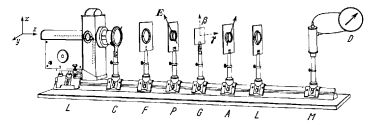
\includegraphics[width=0.6\textwidth]{bilder/glimmer.JPG}\\
		\footnotesize\sffamily\textbf{Quelle:} Pohl \cite{pohl}, Seite 121
	\end{tabular}
	\caption{Versuchsanordnung zur Herstellung von elliptisch polarisiertem Licht}
	\label{fig:glimmer}
\end{figure}
Aus dem Kondensor $C$ fällt angenähert parallel gebündeltes Licht durch einen Farbfilter $F$ (der mononchromatisches Licht erzeugt) auf einen Polarisator $P$, dessen Schwingungsebene durch den Zeiger \emph{E} gekennzeichnet und unter $\unit[45]{^\circ}$ zur Vertikaten gerichtet ist. Das linear polarisierte Licht trifft senkrecht auf das doppelbrechende Glimmerplättchen $G$, welches das Licht in den 2 senkrecht stehenden außerordentlichen Teilbündeln zerlegt. Das im Kristall schnellere hat eine vertikale, das langsamere eine horizontale Schwingungsebene. Durch die relativ große Dicke des Kristalls sind nach dem Austritt aus der doppelbrechenden Glimmerplatte Gangunterschiede für die beiden Wellen von mehr als $2 \pi$ möglich.\\ \\
Infolge des Gangunterschiedes setzen sich die beiden senkrecht zueinander schwingenden Lichtbündel zu einem elliptisch polarisieren Lichtbündel zusammen\footnote{Die Zusammensetzung zweier zueinander senkrecht stehenden Sinusschwingungen mit gleicher Frequenz ergibt elliptische Bahnen.}.\\ \\
Zum Nachweis der Polarisationsart ist der Analysator $A$ eingebaut worden, das von ihm durchgelassene Licht fällt auf eine Linse $L$, die auf dem Strahlungsmesser $M$ abbildet. Es soll dann die Abhängigkeit der Intensität für verschiedene Winkel $\psi$ zwischen den Schwingungsebenen des Analysators und Polarisators untersucht werden.
\item \textbf{Zirkulär polarisiertes Licht} erhält man mit der gleichen Versuchsanordnung wie für das elliptisch polarisierte Licht, schließlich ist zirkulär polarisiertes Licht ein Sonderfall. Bedingung dafür ist, dass eine Phasendifferenz von $\frac{\pi}{2}$ und ein Gangunterschied von $\frac{\lambda}{4}$ zwischen den beiden durch das Glimmerplättchen $G$ verursachten außerordentlichen Strahlen besteht. Diesen Gangunterschied kann man durch die Dicke der Glimmerplatte bewirken, man benutzt dafür ein sogennantes $\frac{\lambda}{4}$-Blatt, wobei $\lambda$ die Wellenlänge des (monochromatischen) Lichtes ist.
\end{itemize}
\subsection{Aufgabe 2: Differenz der Brechungsindizes}
Es soll in dieser Aufgabe die Differenz der Brechungsindizes $\Delta n$ für das Glimmerplättchen mit 2 Methoden bestimmt werden.
\begin{enumerate}
\item \textbf{Mit apparativen Daten bei zirkular polarisiertem Licht}\\ \\
Aus der Definition der Differenz der Brechungsindizes
\begin{equation*}
\Delta n=n_{a1}-n_{a0}=c \cdot (\frac{1}{v_{\parallel}} - \frac{1}{v_{\perp}})
\end{equation*}
und der Phasengeschwindigkeit
\begin{equation*}
v_p=\frac{\lambda}{T}=\lambda \cdot f
\end{equation*}
folgt
\begin{equation}
\label{eq:aufgabe2}
\Delta n=\frac{\lambda \cdot \Delta \phi}{2 \pi d}
\end{equation}
Für zirkular polarisiertes Licht gilt $\Delta \phi=\frac{\pi}{2}$. Die Wellenlänge $\lambda$ und die Dicke der Platte $d$ werden uns erst im Versuchslabor bekannt sein.
\item \textbf{Mit der elliptischen Polarisation}\\ \\
Es gilt wieder die Beziehung \ref{eq:aufgabe2}. Jedoch ist die Phasenverschiebung unbekannt, lässt sich aber anhand der Messungen der Intensitätsverteilungen bestimmen. Aus dem Musterprotokoll \cite{vorbereitung1} gilt:
\begin{equation*}
\Delta \phi = 2 \arctan\left(\sqrt{\frac{T}{L}}\right)
\end{equation*}
wobei $T$ die Taillenweite und $L$ die Länge des Graphen im Polardiagramm ist.
\end{enumerate}
\subsection{Aufgabe 3: Farbänderung bei Drehung des Analysators}
In diesem Versuch werden nun Glimmerplättchen und Klebefilmbilder (aus Tesa) mit weißem, polarisiertem Licht, welches aus vielen Wellenlängen besteht, bestrahlt. Da das Glimmerplättchen und, wie wir im Versuch sehen werden, auch die Klebefilmbilder doppelbrechend sind, erfahren die verschiedenen Wellenlängen unterschiedliche Phasenverschiebungen. Es entsteht elliptisch Polarisiertes Licht. Den Analysator lässt je nach Einstellung unterschiedliche Farben unterschiedlich stark durch, wird dieser also gedreht, so sollten sich die Farbkomponenten des Bildes ändern.
\subsection{Aufgabe 4: Spannungsdoppelbrechung an Plexiglas}
Auch in isotropen Medien kann es durch mechanisch Spannung zur Doppelbrechung kommen, dabei kommt es durch die mechanische Spannung zu elastischer Verformung  im Inneren. Es bildet sich eine optische Achse entlang der Richtung der angelegten Spannung. Im allgemeinen gilt dabei, das die Ausprägung der Doppelbrechung proportional zu stärke der Spannung ist. In diesem Versuch wird eben dieser Effekt an Plexiglas demonstriert.\\
Mit einem Polarisationsfilter lässt sich die Farbänderung im Material beobachten, wobei unterschiedliche Farben, unterschiedlichen Spannungen entsprechen.
\newpage
\bibliographystyle{plain}
\bibliography{quellen}

\end{document}